\documentclass[12pt]{article}

\usepackage[english]{babel}
\usepackage[utf8x]{inputenc}
\usepackage{pdfpages}
\usepackage{lastpage} % Required to determine the last page for the footer
\usepackage{extramarks} % Required for headers and footers
\usepackage{graphicx} % Required to insert images
\usepackage{listings} % Required for insertion of code
\usepackage{courier} % Required for the courier font
\usepackage{color}
\usepackage{grffile}
\usepackage{float}

% Margins
\topmargin=-0.45in
\evensidemargin=0in
\oddsidemargin=0in
\textwidth=6.5in
\textheight=9.0in
\headsep=0.25in
\fboxsep=0mm%padding thickness
\fboxrule=2pt%border thickness

\linespread{1.1} % Line spacing

\newcommand{\Title}{Software requirement specification} % Assignment title
\newcommand{\Class}{Cos\ 301} % Course/class
\newcommand{\pd}{Post-Doctoral}
\newcommand{\ssr}{Soft\color{green}{Serve }\color{black}}
\begin{document}

	\vspace{4em}
	
	\begin{center}%
	
		\begin{figure}[ht!]
			\centering
			
\includegraphics{./Pictures/logo.png}
	 	\end{figure}
		\LARGE \bf \Title \\
		{\bf Version 0.5}\\[4em]
	  	\LARGE {\bf \ssr  Group }\\[1em]
	  	\LARGE {\bf Members:}\\[2em]
	  	\large
	     Kgothatso Phatedi Alfred Ngako	(12236731) \\[1em]
	     Tokologo “Carlo” Machaba			(12078027) \\[1em]
	     Mathys Ellis						(12019837) \\[8em]
	    
	\end{center}%
	
	%\newpage
		%{\LARGE \bf Change log}\\[2em]
		
		%\begin{tabbing}
			%\hspace*{2.5cm}\=\hspace*{2.5cm}\=\hspace*{8cm}\=\hspace*{3cm} \kill
	\begin{center}
		\begin{tabular}{|l|p{1.4cm}|p{8cm}|p{2.8cm}|}
			\hline
			\multicolumn{4}{|c|}{\bf Change log} \\
			\hline
			\bf Date & \bf Version & \bf Description & \bf Person \\
			\hline
			10/02/2014 & v 0.0 & Document created & Mathys Ellis \\
			\hline
			02/03/2014 & v 0.1 & Added to glossary & Mathys Ellis \\
			\hline
			04/03/2014 & v 0.2 & Added Integration requirements, Architecture constraints, Functional requirements introduction   & Alfred Ngako \\
			\hline
			05/03/2014 & v 0.3 & Added Introduction, Vision, Background, Access Channel requirements & Carlo Machaba \\
			\hline
			06/03/2014 & v 0.4 & Added domain objects, open issues. Modified some sections  & Alfred Ngako \\
			\hline
			06/03/2014 & v 0.5 & Added quality requirements, methodology, scope and limitations  & Mathys Ellis \\
			\hline
			08/03/2014 & v 0.6 & Added some wrapping to the change log which is now a table  & Alfred Ngako \\
			\hline
			
		%\end{tabbing}
		\end{tabular}
	\end{center}
	\newpage
		\tableofcontents
			
		\listoffigures
	\newpage
	\section{Introduction} %Carlo
	A Post-Doctoral fellow is a person who conducts research after they have completed their PhD, with the aim of deepening their knowledge in a specific field. The University of Pretoria supports such research opportunities in order to the increase research output of the University. Post-Doctoral fellows who conduct their research at the University of Pretoria do so under the supervision of a staff member of the University and their research may be privately or internally funded. This is a growing field in Universities around South Africa. Thus a lack in the IT services for the application management of Post-Doctoral fellow has been spotted by SoftServe.  
	\vspace{0.2in}

		\subsection{Purpose:}
		\vspace{0.2in}
		This Software Specifications Requirements document serves the purpose of providing a detailed overview of the non-functional and functional requirements as well the goals that SoftServe's Post-Doctoral application management system wishes to satisfy. Further it defines the abstract interaction of stakeholders with the system. Thus this document serves as a contract between SoftServe and the client, Mrs Cathy Sandis of the DRIS of the University of Pretoria.
	
		\vspace{0.2in}
	
		\subsection{Document Conventions:}
		\vspace{0.1in}
		\begin{itemize}
			\item Documentation formulation: LaTeX
			\item ERD Crow-Foot notation
			\item UML 2.0
		\end{itemize}
	
		\vspace{0.2in}
	
		\subsection{Project Scope:}
		\vspace{0.2in}		
		The scope of the project is to design a Post-Doctoral application management system where prospective or current Post-Doctoral fellows can apply for or renew fellowships at the University of Pretoria. The system will then further allow the management of such applications/renewals till the end of the application process. The end is defined as: DIRS have approved the application and have notified the CSC and Finance department. The system will replace the current paper based system currently in place. The system will be designed so to allow for future integration with the current student and personnel management system, PeopleSoft, employed by the University of Pretoria. Though the scope of this SRS document will be to make the system and have it independent of any other system.
		\vspace{0.2in}
	
		\subsection{References:}
		\vspace{0.1in}
		\begin{itemize}
			\item Dr.Phol, K., 2010, \textit{Requirements Engineering: Fundamentals, Principles, and Techniques}, Springer, Heidelberg.
		\end{itemize}			
	
	\vspace{0.5in}
	
	\section{Vision} %Carlo	
	\vspace{0.2in}
	The client needs a system which can make the management of the application and renewal processes of Post-Doctoral fellowships more effective, reliable, secure and audit-able. Together the client and SoftServe have envisioned a system that will make use of a centralised user friendly web interface that will be used by the prospective fellows and all the stakeholders involved in the application and renewal processes. The system will have various sections that handle the different stages in the process. The system will need to automate the transitions between phases by forwarding the required information to the next stakeholder in the process and notifying them via a email notification. The system will also need to provide reporting facilities for the information stored by the system. As well as progress tracking with regards to any application or renewal. The system data needs to be centralised to ensure that any information used by system is cohesive and valid for any stakeholder who accesses it. By introducing a digital system that is not paper based, the client hopes that the application and renewal processes will be easier to track and manage.
	\vspace{0.5in}
	
	\section{Background} %Carlo
	\vspace{0.2in}
	The current Post-Doctoral application and renewal processes are paper based thus there are a number of drawbacks, mainly due to human error. One such drawback is that there is no audit trail when it comes to the different stakeholders input involved in approving or declining the applications. Another involves the minutes of Post-Doctoral committee meetings which are often misplaced or typed in an inconsistent manner making it hard to recall what has been discussed in the meetings that evaluate prospective applications and renewals. Access to documents is also a problem since they are usually hard copies that change hands constantly thus the process of getting hold of the documents is long and often tedious if not made impossible if they are lost. Reporting on the information of fellows, renewals and even communication with already approved fellows is also problematic, because the current system is not centralised. Therefore gathering all the information required to generate the reports is difficult or even impossible. This is where the client Mrs Cathy Sandis saw a potential area that could be optimised by the implementation of digitalised system. This is where the SoftServe group was brought into the picture. 
	\vspace{0.5in}
	
	\newpage
	\section{Methodology} %Mathys
	\vspace{0.2in}
	
	This document was created using the requirement elicitation techniques and requirement definitions specified in Klaus Pohl’s book Requirements Engineering: Fundamentals, Principles, and Techniques [Dr.Phol, K., 2010].
	The requirements were elicited from the following sources:
	\begin{itemize}
		\item Numerous interviews with the client
		\item Collecting and analysing various documents such as:
		\begin{itemize}
			\item The initial project request document
			\item Application forms
			\item Renewal forms
			\item CV templates
			\item Approval and recommendation forms			 
		\end{itemize}		
		\item Online research into UP Post doctoral applications
		\item Correspondence with the UP IT department
	\end{itemize}	
	
	\vspace{0.5in}
	
	
	\newpage
		\section{Stakeholders} %Mathys
		\vspace{0.2in}
		
		The stakeholders that will engage or be engaged by the system are listed below:
		
		There are three categories under which stockholders can fall:
		\begin{itemize}					
			\item External:
			These are stakeholders that do not have a PeopleSoft account or are fellows.
			\begin{itemize}		
				\item \textbf{Prospective fellow} - A person who wishes to renew or apply for a research position/fellowship.
				\item \textbf{Referee} - A person who is identified by a Prospective fellow as a referral.
			\end{itemize}
			
			\item Internal individuals:
			These are stakeholders that do have a PeopleSoft account and are individual members of staff.
			\begin{itemize}	
				\item \textbf{Grant holder} - The person who is a fellow's supervisor and a member of staff at the University of Pretoria. This is person is known also the applicant.
				\item \textbf{HOD} - The head of the department of which a Grant holder is a member.					
			\end{itemize}
			\item Internal groups:
			These are stakeholders that do have a PeopleSoft account and are a group of staff members.
			\begin{itemize}	
				\item \textbf{Dean's office} - The dean and deputy dean of the faculty under which the department which the Grant Holder is a member of.
				\item \textbf{DRIS} - The department of Research and Innovation Support at the University of Pretoria. This stakeholder oversees the application and renewal processes.
				\item \textbf{Post-doctoral committee} - The committee who evaluates any post-doctoral fellowship applications and renewals.
				\item \textbf{CSC} - The client service centre of the University of Pretoria.
				\item \textbf{Finance} - The department of finance at the University of Pretoria.	
			\end{itemize}
		\end{itemize}
		\vspace{0.5in}
	
	\newpage
	\section{Architecture requirements}
		\subsection{Access channel requirements} %Carlo
		\vspace{0.2in}
		All stakeholders: Will access the system through a HTML 5 web browser client that is locally installed on a user's computer system or mobile platform. Support for HTML 4.0.1 will also be implemented. The web interface will allow different stakeholders access to different sections of the system based on the roles assigned to their accounts.   

		\vspace{0.2in}
		
		\subsection{Quality requirements} %Mathys
		\vspace{0.2in}
		
		\subsubsection{Availability:}
				
		\begin{flushleft}
		
		The system's availability on designated networks will depend on the availability of the University of Pretoria's servers that host the system. If the University of Pretoria's servers hosting the system are active and provide access over a designated network then the system must be available over that designated network. The designated networks are defined as the internet and the campus network of the University of Pretoria.
		
		\end{flushleft}
		
		\vspace{0.1in}
				
		\subsubsection{Security requirements}
		
		\begin{flushleft}
		
		The system will need to be fully secured since the system deals with confidential information such as person information, application statuses, financial data and meeting information. Also since the systems main goal is to provide stable and audible application and renewal process flow the system may not be vulnerable to data tampering or any tampering whatsoever. \\
		\vspace{0.1in}
		  
		The system will have to provide different security roles to the registered users on the system. Any number of roles should be assignable to any user by a administrator with the correct role to allow for flexibility. 
		But in essence a stakeholder may only have access to their section of the application process. The system administrator should be able to view all the sections in the system and should be able to modify them except where they may not.
		
		\end{flushleft}
		
		\vspace{0.1in}
		
		\subsubsection{Scalability requirements}
		
		\begin{flushleft}
		
		The current aim is to create a scalable system that can support 500 to 1000 applicants per year with possible growth. This is in line with the figures given by the client and the growth in the research sector of the university.\\
		\vspace{0.05in}
		
		The system needs to be scalable in regard to the following factors:
		\begin{itemize}
		
		
		\item\textbf{Performance:} This is regarded as the speed and responsiveness of the system.		
		The system needs to be handle report queries in less than 10 seconds. It should be able to handle any application section processing in less than 3 seconds.\\
		
		\item\textbf{Storage:} This is regarded as the growth and shrinking of the data that is stored.
		The system will need to be able to handle a database that is in the range of 1 GB to 15 GB that has the potential to grow even larger.  The reason for this stems from the requirement that the system will support archival functionality and archived data will store the data for long periods of time.\\
		 
		\item\textbf{Concurrency:} This regarded as the amount of active users on the system at the same time.		
		The system will need to support at least 100+/- concurrent users efficient and effectively since the system requires multiple stakeholders to part take in the application process while there can be multiple applications occurring at the same time.\\ 
		 
		\end{itemize}
		\end{flushleft}
		\vspace{0.1in}
		
		\subsubsection{Testability:}
				
		\begin{flushleft}
		
		The system must be testable. This will be done using unit testing and following the test plan that will be laid out in the testing document of this project.\\
		
		\vspace{0.1in}
		
		Unit testing will test each unit in regard to:
		\begin{itemize}
		
		\item\textbf{Preconditions}
		\item\textbf{Post conditions}
		
		\end{itemize}
		
		The project will also have two phases of testing:
		
		\begin{itemize}
		
		\item\textbf{Offline:} This is the initial phase of testing and debugging which will be done with pseudo data.
		\item\textbf{Online:} This is the final phase of testing and debugging which will be done with active real time data.
		
		\end{itemize}
		
		\end{flushleft}
		
		\vspace{0.1in}
		
		\subsubsection{Auditability:}
				
		\begin{flushleft}
		
		The system needs to provide an audit trail of all critical actions that occur in the system. Critical actions are considered: user account management operations, login action, logout action and any operation by a user that leads to a change in application data of a particular prospective fellow.\\
		
		\vspace{0.1in}
		
		The Audit trail will be in the form of a read-only table stored in the database. It can only be viewed by a user with the correct security role. The system is the only entity that can modify the audit trail where this modification can only be the addition of entries.
		
		\end{flushleft}
		\vspace{0.1in}	
		
		\subsubsection{Usability requirements}
		
		\begin{flushleft}
		
		The primary language of the system will be South African English. Any other language support is not considered part of the requirements but the system will be designed to allow for such development in the future.\\
		
		\vspace{0.1in}
				
		The system's UI will only consider 2 types of user categories with regard to usability:
		
		\begin{itemize}
		
		\item\textbf{Trained user:}
		
		This type of user will have to have training in understanding how the system functions and how to use it. Their computer skills will be assumed to be in the range of basic to intermediate. Thus the user interface can allow for certain complexities but these complexities must be kept at a minimal. This user will be regarded as a system administrator.  The stakeholders who fall under this category is the DRIS staff members overseeing the application process.
		
		\item\textbf{Normal user:}
		
		This type of user will have no training. Their computer skills will be assumed to be none or minimal. Therefore the UI that they will have access to will be simplistic and will be as user friendly as possible. The stakeholders that fall under this category will be Prospective fellows, Grant holders, HODs, Deans and Post-doctoral committee members.
		
		\end{itemize}
		
		\end{flushleft}
		
		\vspace{0.2in}	
		
		
		\subsection{Integration requirements} %Alfred
		\vspace{0.2in}
		The system has to integrate with the following systems:
		\begin{itemize}
			\item Must be able to create exportable data packages containing the information of approved fellowships that can easily be loaded into the CSC PeopleSoft system. 
			\item Must be able to query CSC PeopleSoft system to retrieve the account information of internal individuals/group Stakeholders to create a uniform login experience.
			\item Must assign Prospective fellows with a id number in such a way that is integrable with UP Emplid. SoftServe suggests: "f" + 8 digit code. 
			\item Must be able to access and utilize the NRF researcher ratings.
		\end{itemize}
		\vspace{0.2in}
		
		\subsection{Architecture constraints} %Alfred
		\vspace{0.2in}
		The following architecture constraints have been selected as being suitable for the system.
		\begin{enumerate}
			\item Database technology: MySQL
			\item Development technology: Java EE
			\item Web server: Apache Tomcat
			\item Application server: GlassFish 
			\item Web interface protocol: HTTPS
		\end{enumerate}
		\vspace{0.5in}
	
		
	\section{Functional requirements}
		\subsection{Introduction} %Alfred
		\vspace{0.2in}
		This section discusses the functional requirements for the University of Pretoria's Post-Doctoral application management system. Highlighting the scope and limitations that are faced by the system. \linebreak \linebreak
		The required functionality, domain objects and use cases related to the functional requirement will be discussed. 
		\vspace{0.2in}
		
		\subsection{Scope and Limitations/Exclusions} %Mathys
		\vspace{0.2in}
			
		
		\subsubsection{Scope}
		\vspace{0.2in}
		
			\begin{figure}[H]
				\centering				
				\framebox{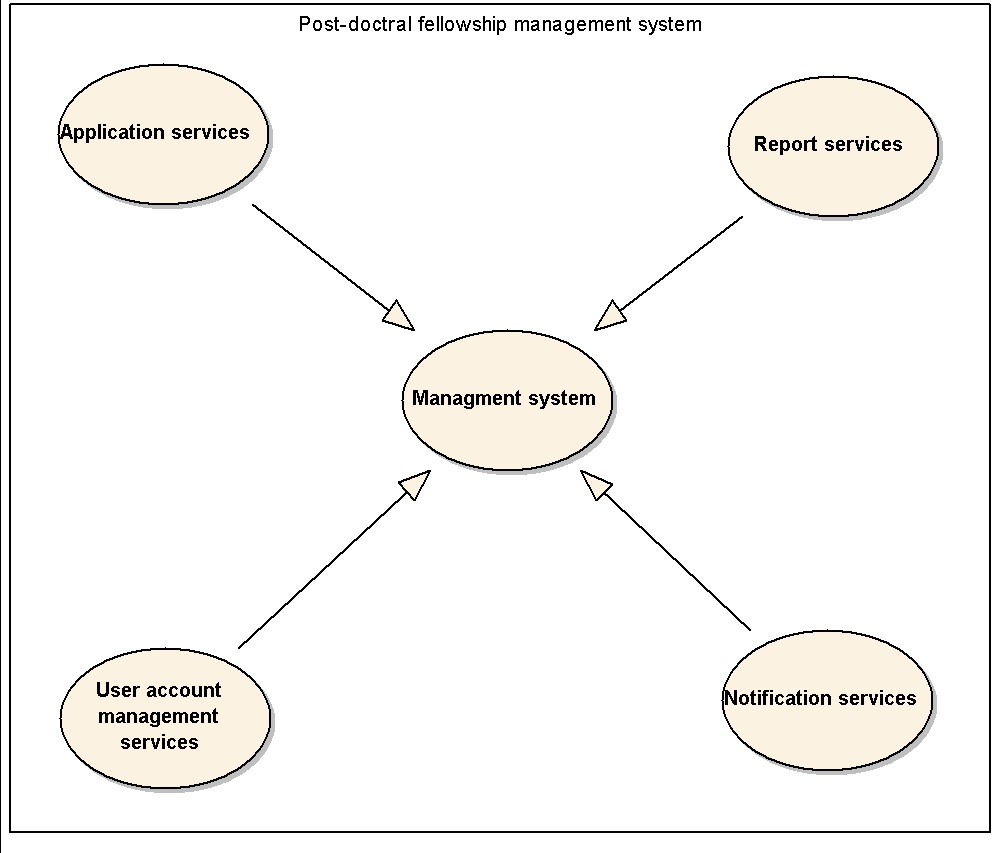
\includegraphics[scale=0.6]{./Pictures/Diagrams/Post-doctral fellowship management system.jpg}}
				\caption{Use case diagram of Post-doctoral fellowship management system}
			\end{figure}
			
			\begin{figure}[H]
				\centering				
				\framebox{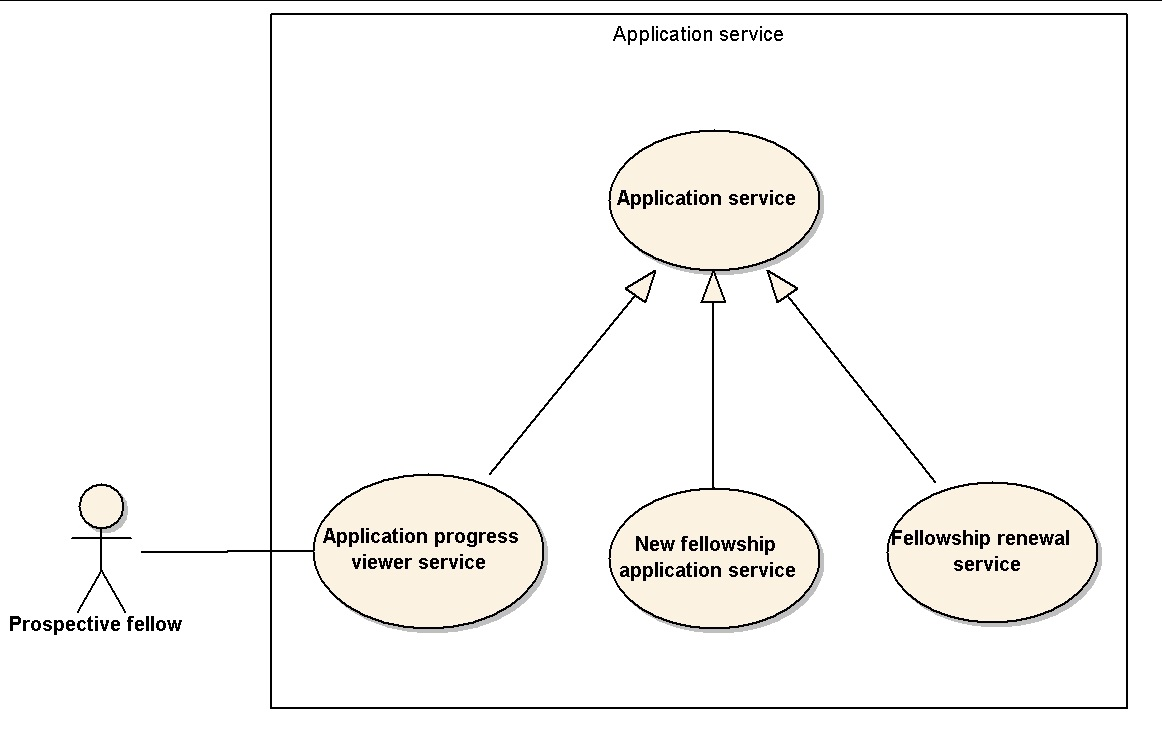
\includegraphics[scale=0.6]{./Pictures/Diagrams/Application service.jpg}}
				\caption{Use case diagram of Application service}
			\end{figure}
									
			\begin{figure}[H]
				\centering				
				\framebox{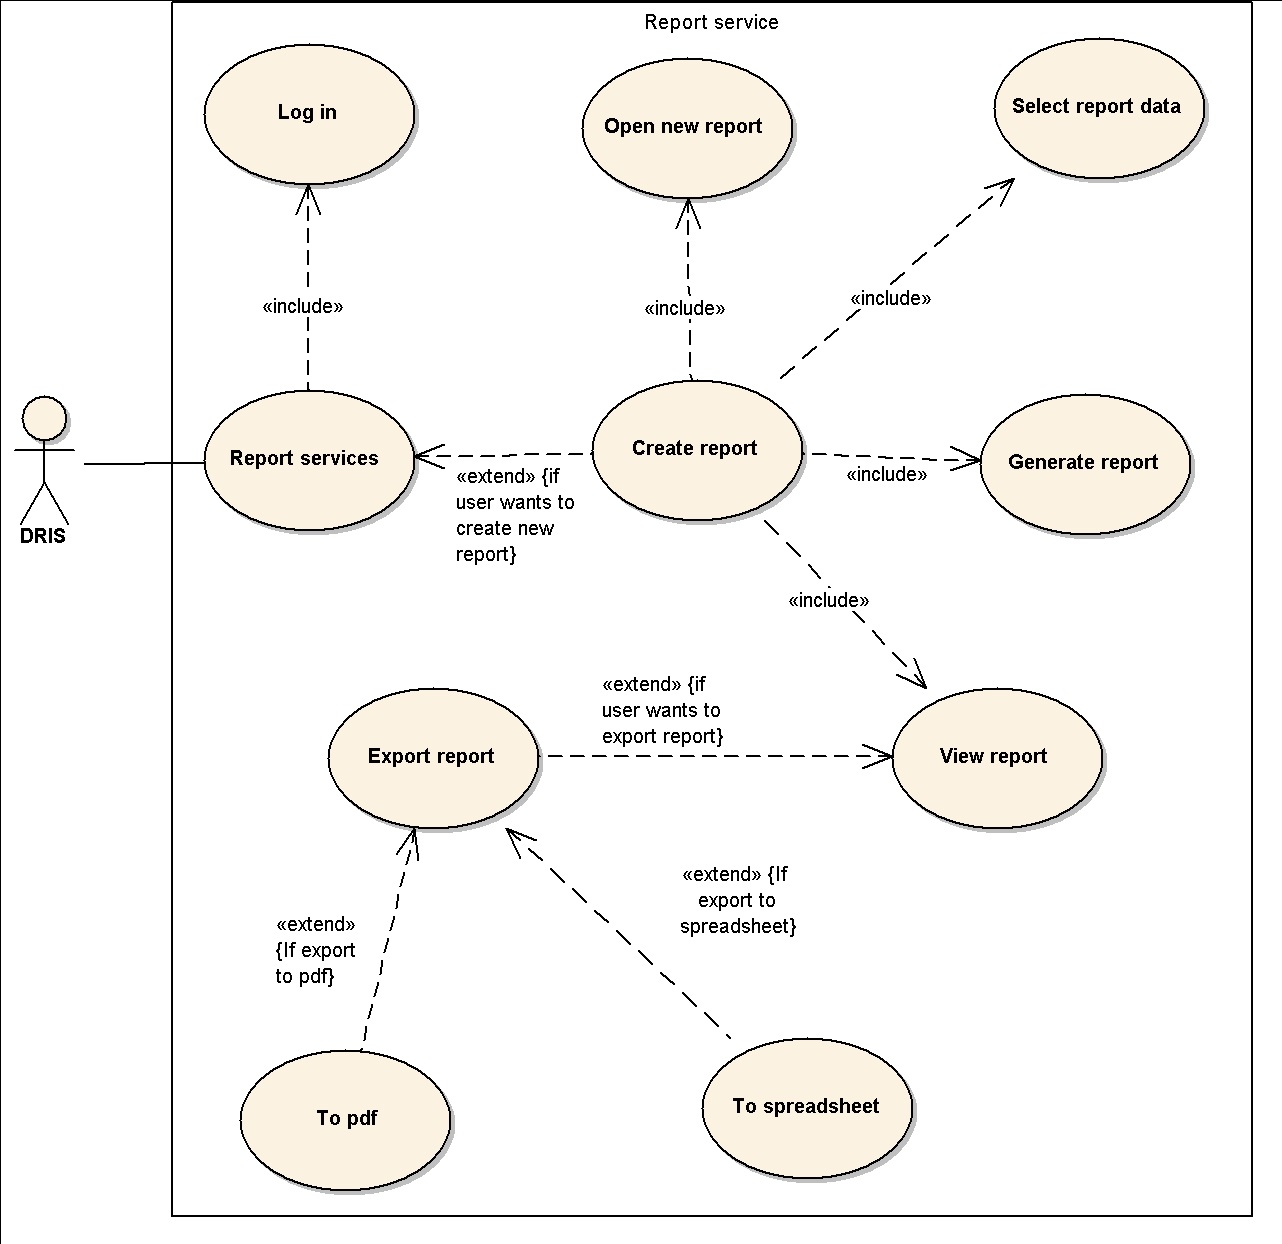
\includegraphics[scale=0.6]{./Pictures/Diagrams/Report service.jpg}}
				\caption{Use case diagram of Report service}
			\end{figure}
			
			\begin{figure}[H]
				\centering				
				\framebox{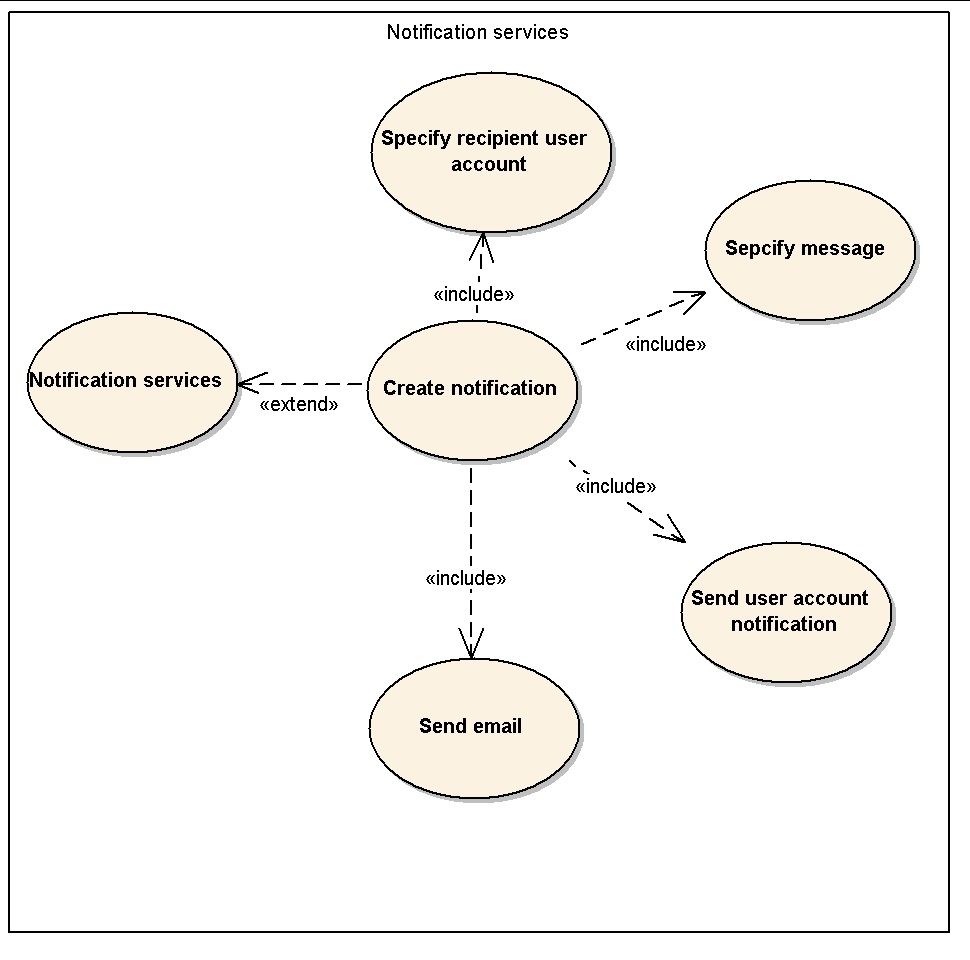
\includegraphics[scale=0.6]{./Pictures/Diagrams/Notification services.jpg}}
				\caption{Use case diagram of Notification services}
			\end{figure}
			
			\begin{figure}[H]
				\centering				
				\framebox{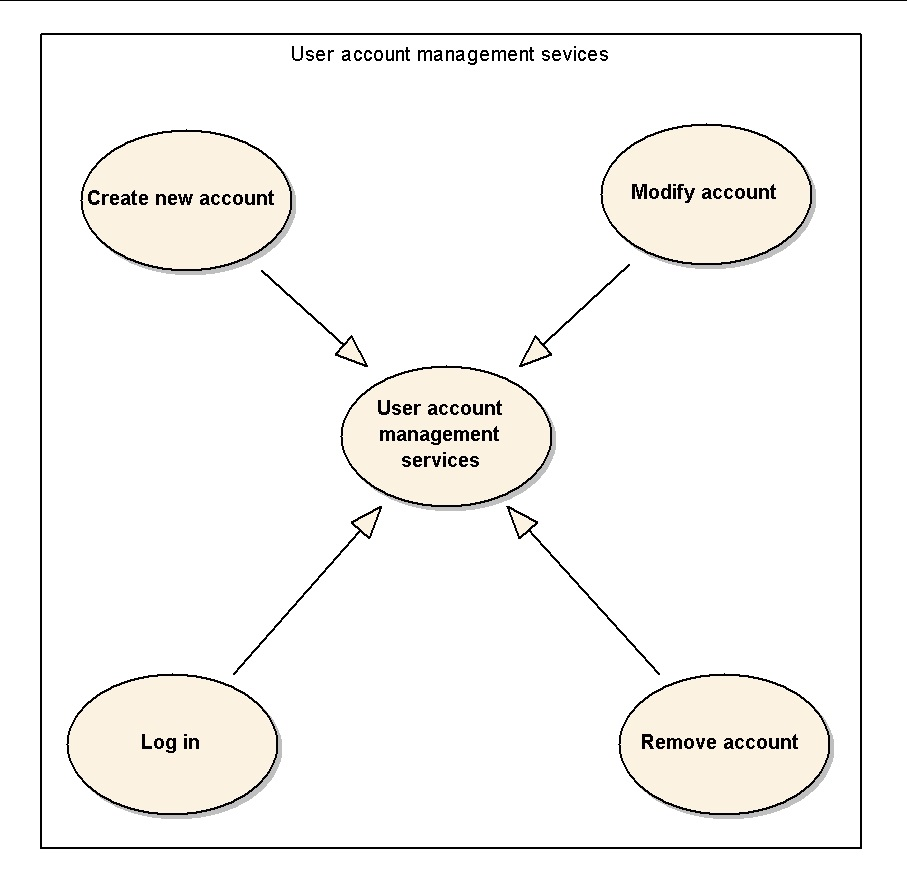
\includegraphics[scale=0.6]{./Pictures/Diagrams/User account management services.jpg}}
				\caption{Use case diagram of User account management services}
			\end{figure}
			
			\begin{figure}[H]
				\centering				
				\framebox{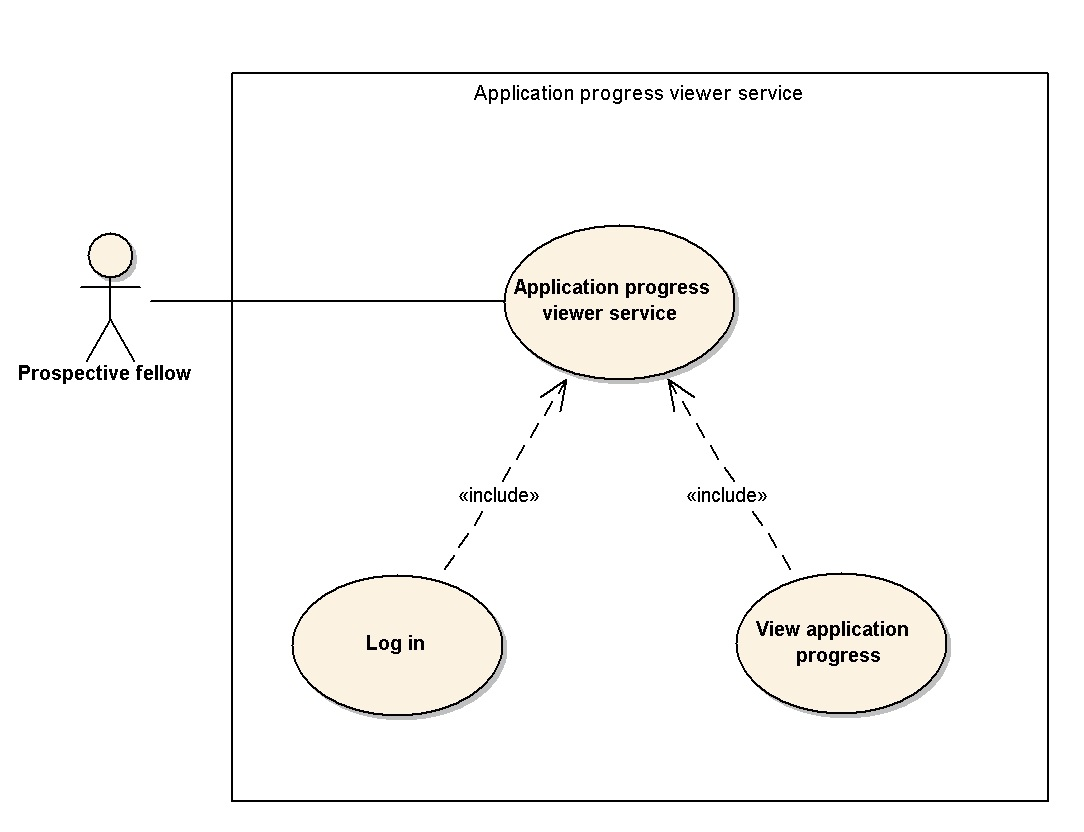
\includegraphics[scale=0.6]{./Pictures/Diagrams/Application/Application progress viewer service.jpg}}
				\caption{Use case diagram of Application progress viewer service}
			\end{figure}
			
			\begin{figure}[H]
				\centering				
				\framebox{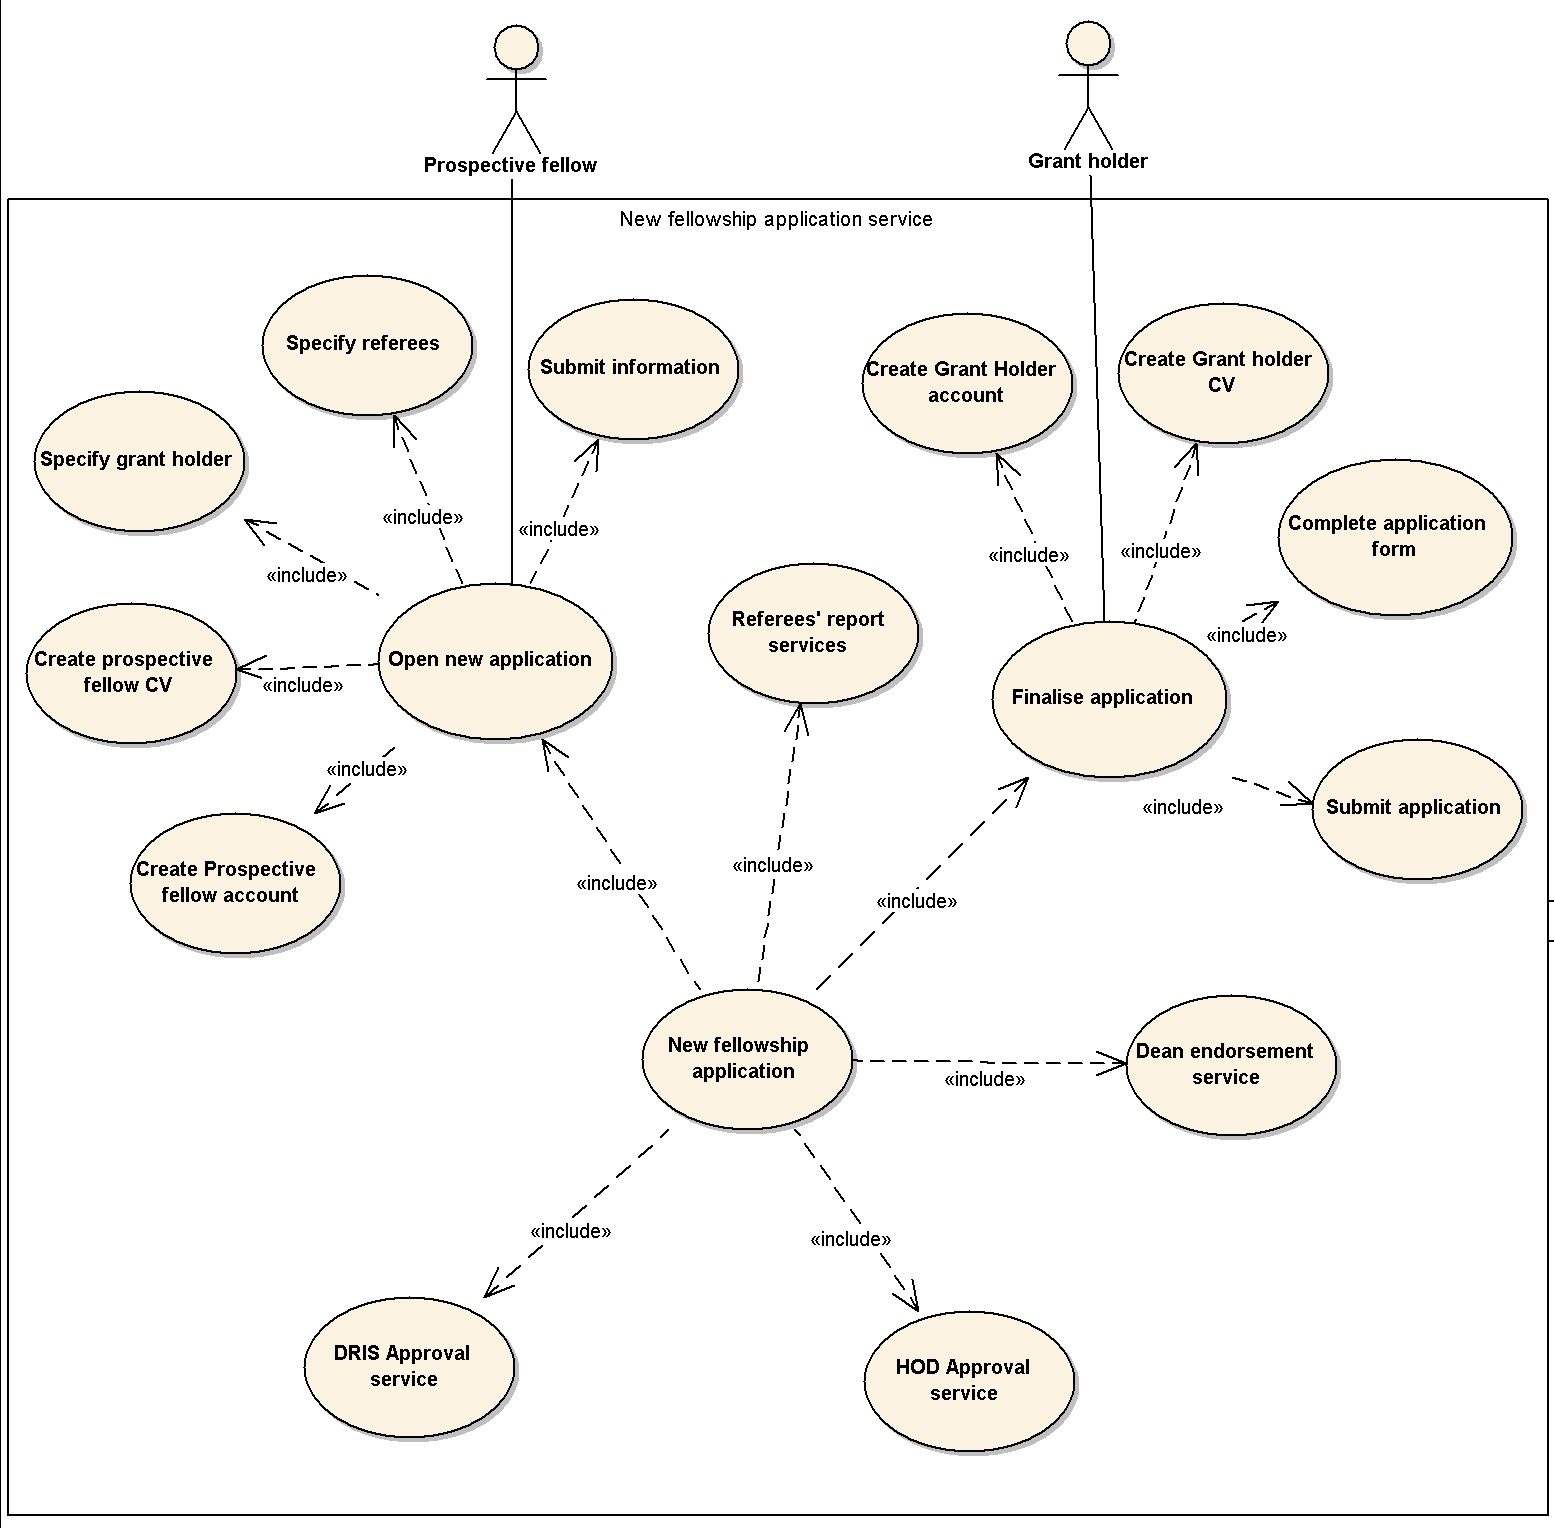
\includegraphics[scale=0.6]{./Pictures/Diagrams/Application/New fellowship application service.jpg}}
				\caption{Use case diagram of New fellowship application service}
			\end{figure}
			
			\begin{figure}[H]
				\centering				
				\framebox{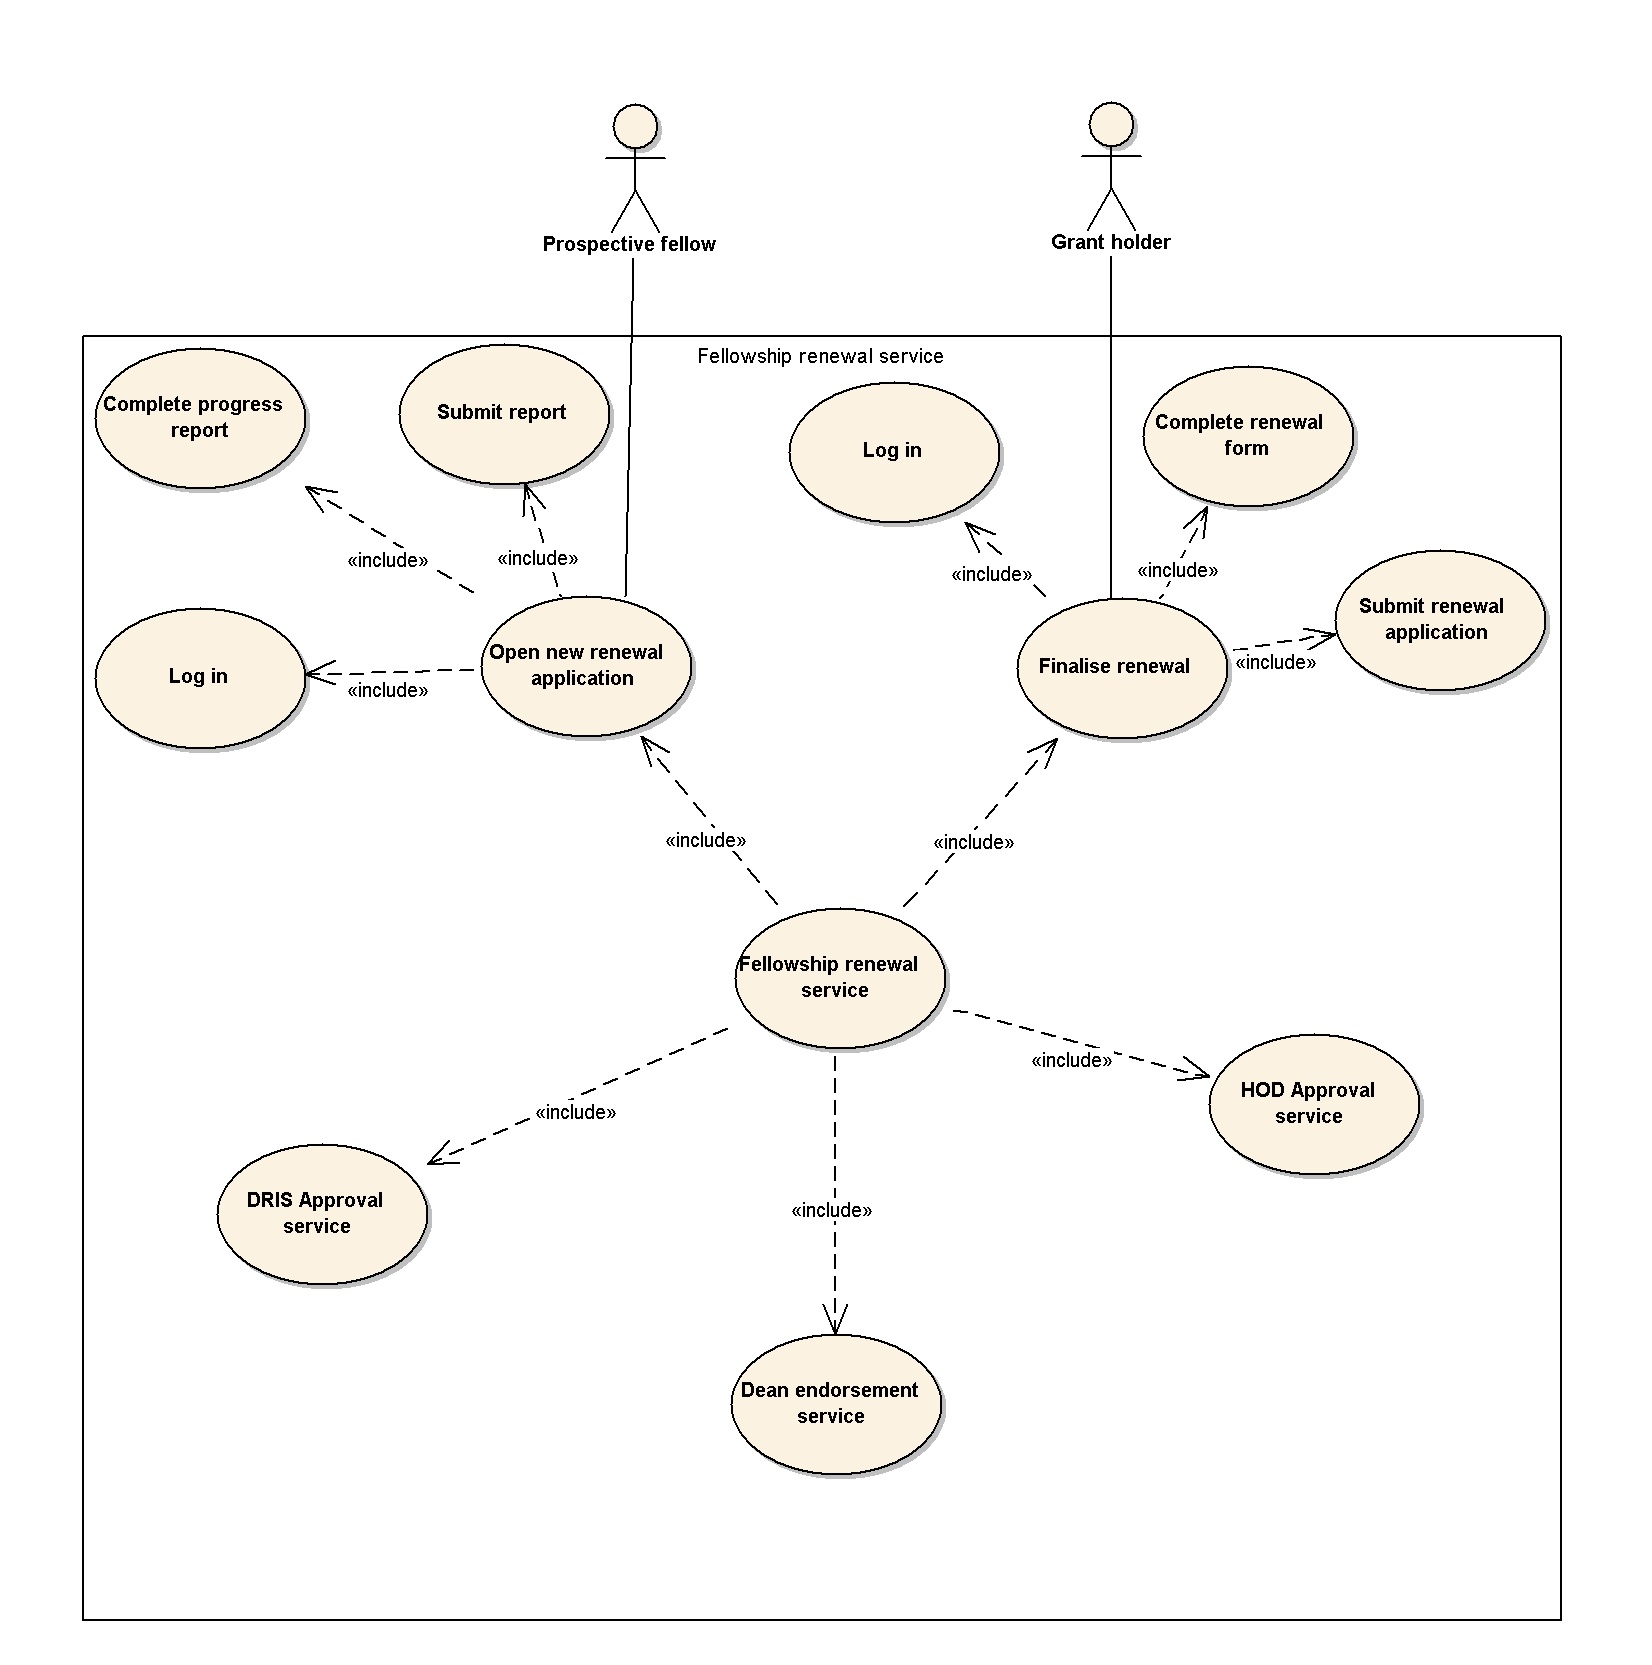
\includegraphics[scale=0.6]{./Pictures/Diagrams/Application/Fellowship renewal service.jpg}}
				\caption{Use case diagram of Fellowship renewal service}
			\end{figure}
			
			\begin{figure}[H]
				\centering				
				\framebox{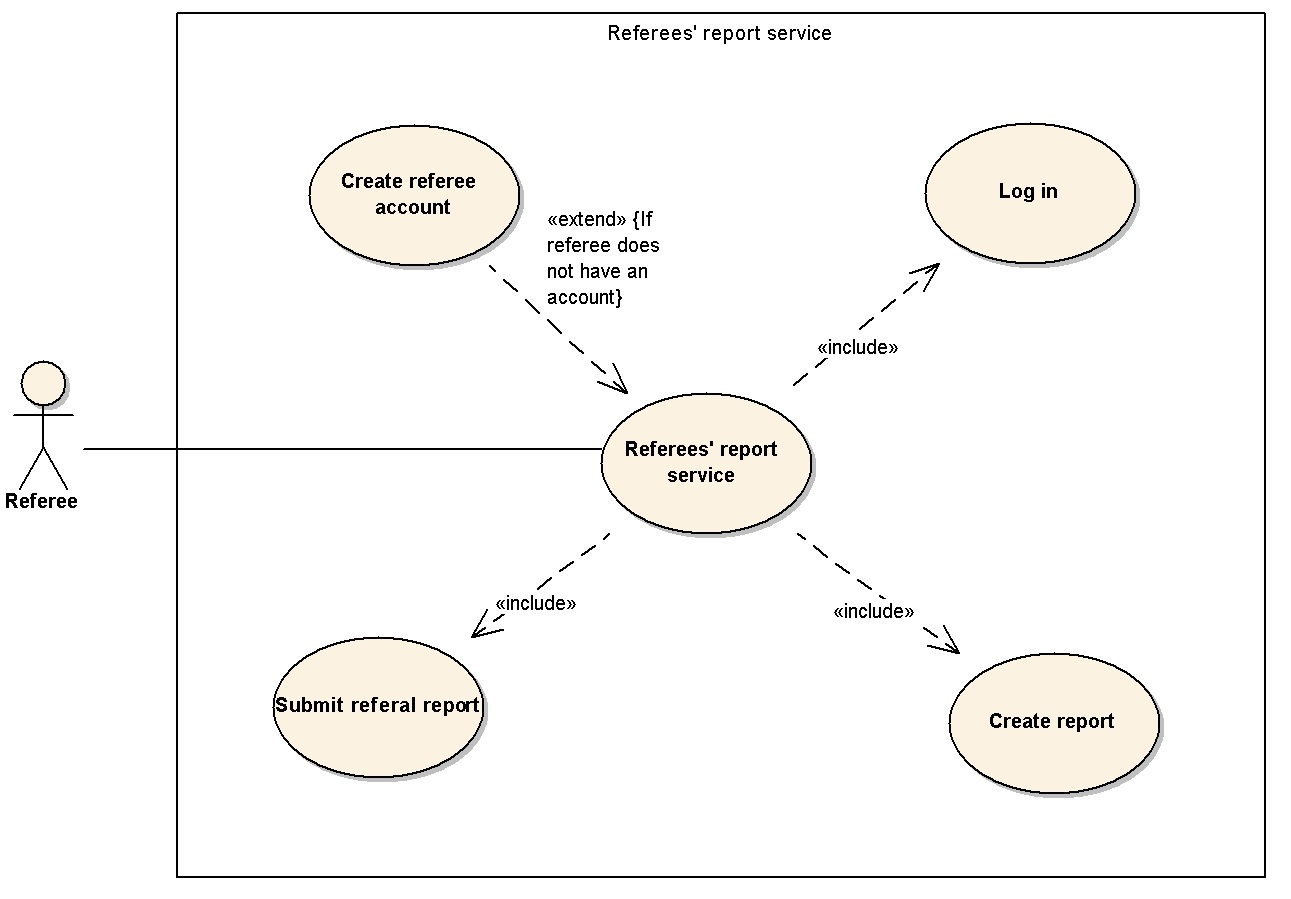
\includegraphics[scale=0.6]{./Pictures/Diagrams/Application/Referees' report service.jpg}}
				\caption{Use case diagram of Referees' report service}
			\end{figure}
			
			\begin{figure}[H]
				\centering				
				\framebox{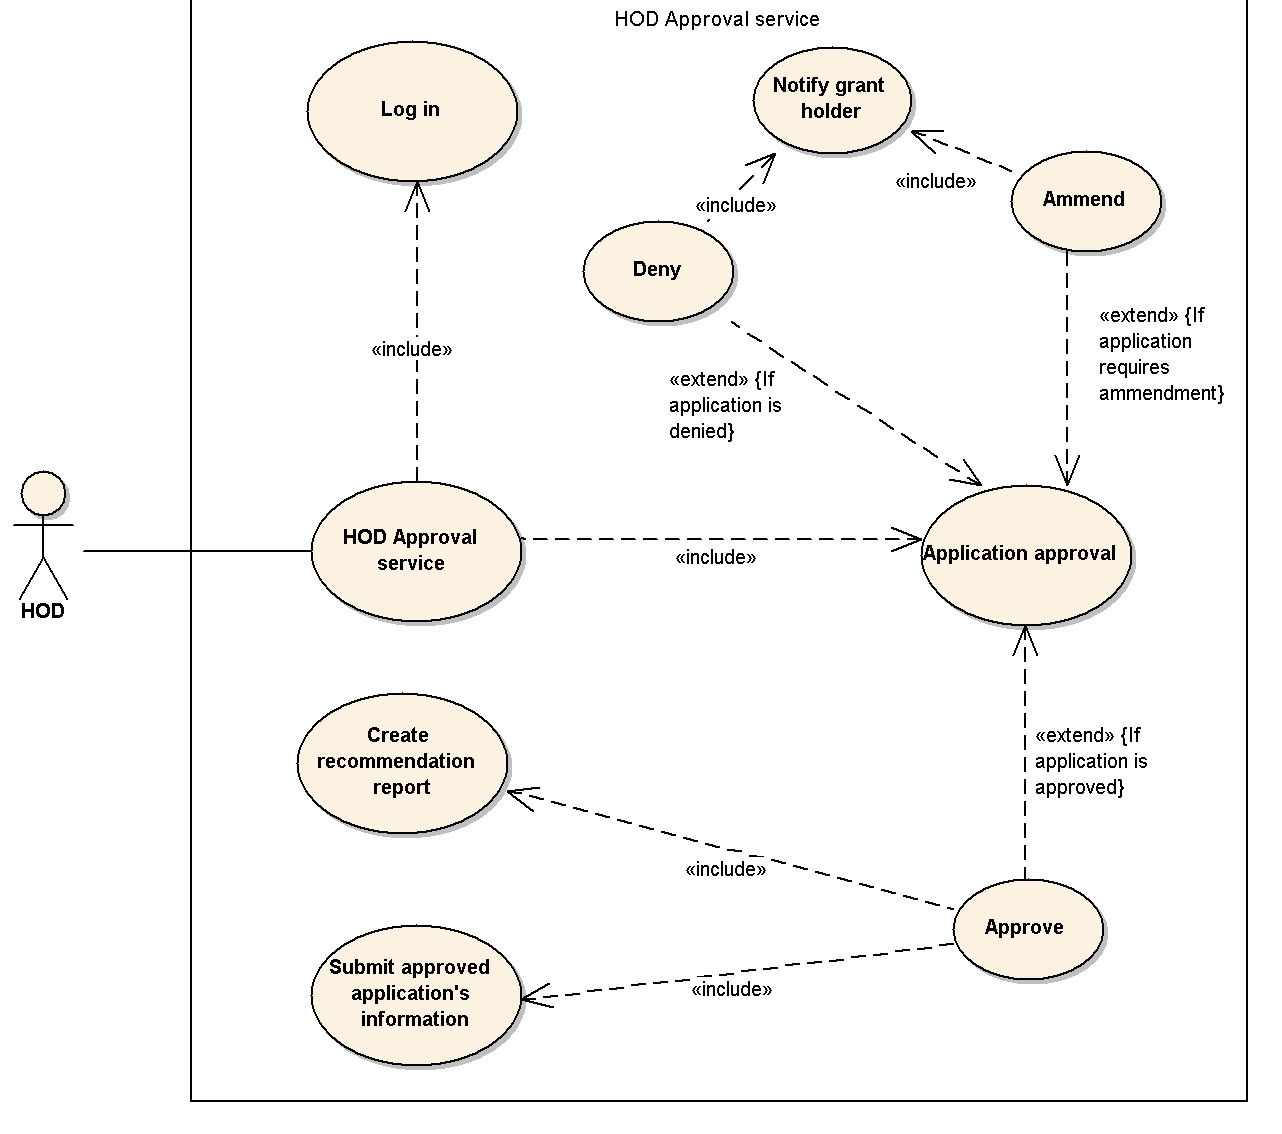
\includegraphics[scale=0.6]{./Pictures/Diagrams/Application/HOD Approval service.jpg}}
				\caption{Use case diagram of HOD Approval service}
			\end{figure}
			
			\begin{figure}[H]
				\centering				
				\framebox{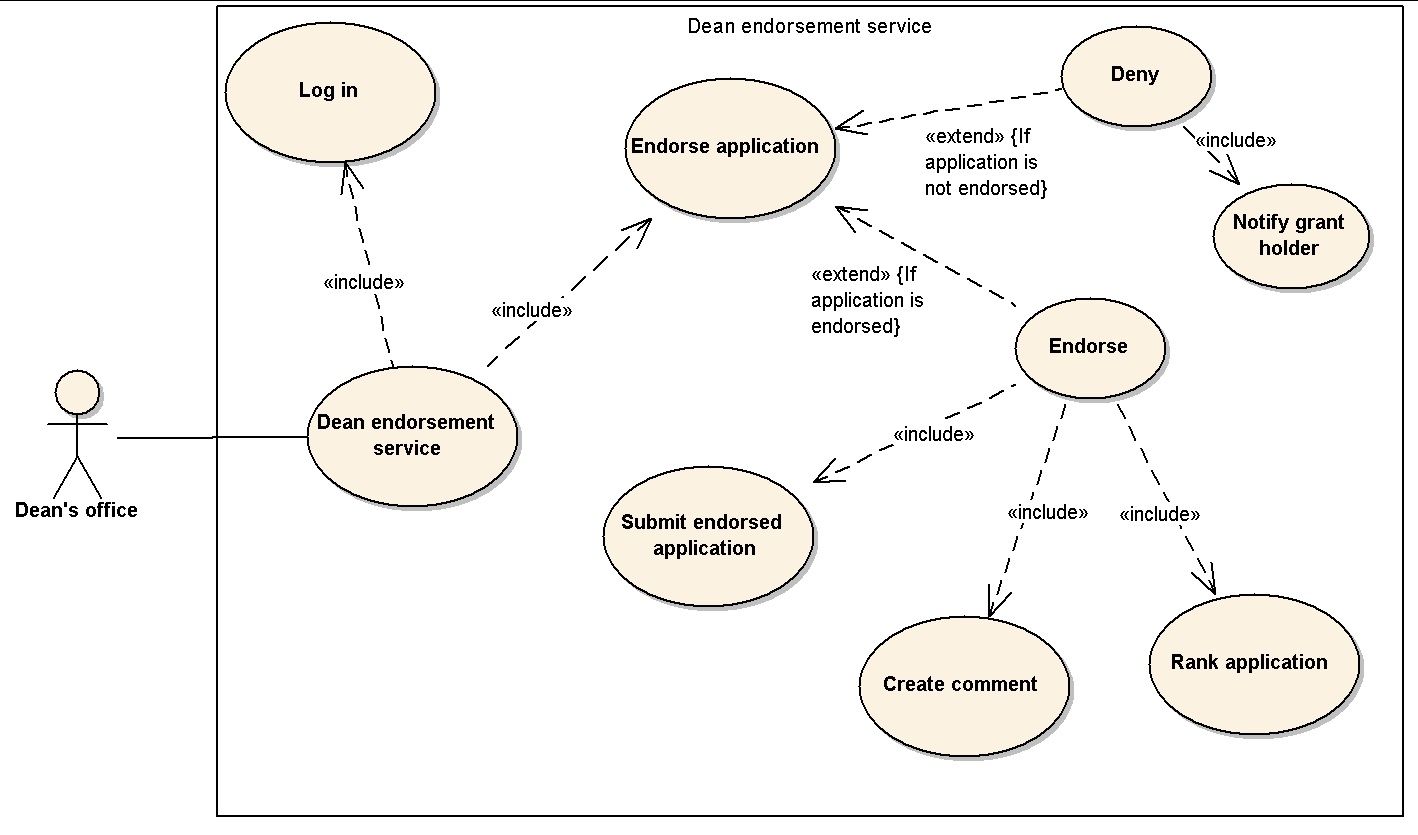
\includegraphics[scale=0.6]{./Pictures/Diagrams/Application/Dean endorsement service.jpg}}
				\caption{Use case diagram of Dean endorsement service}
			\end{figure}
			
			\begin{figure}[H]
				\centering				
				\framebox{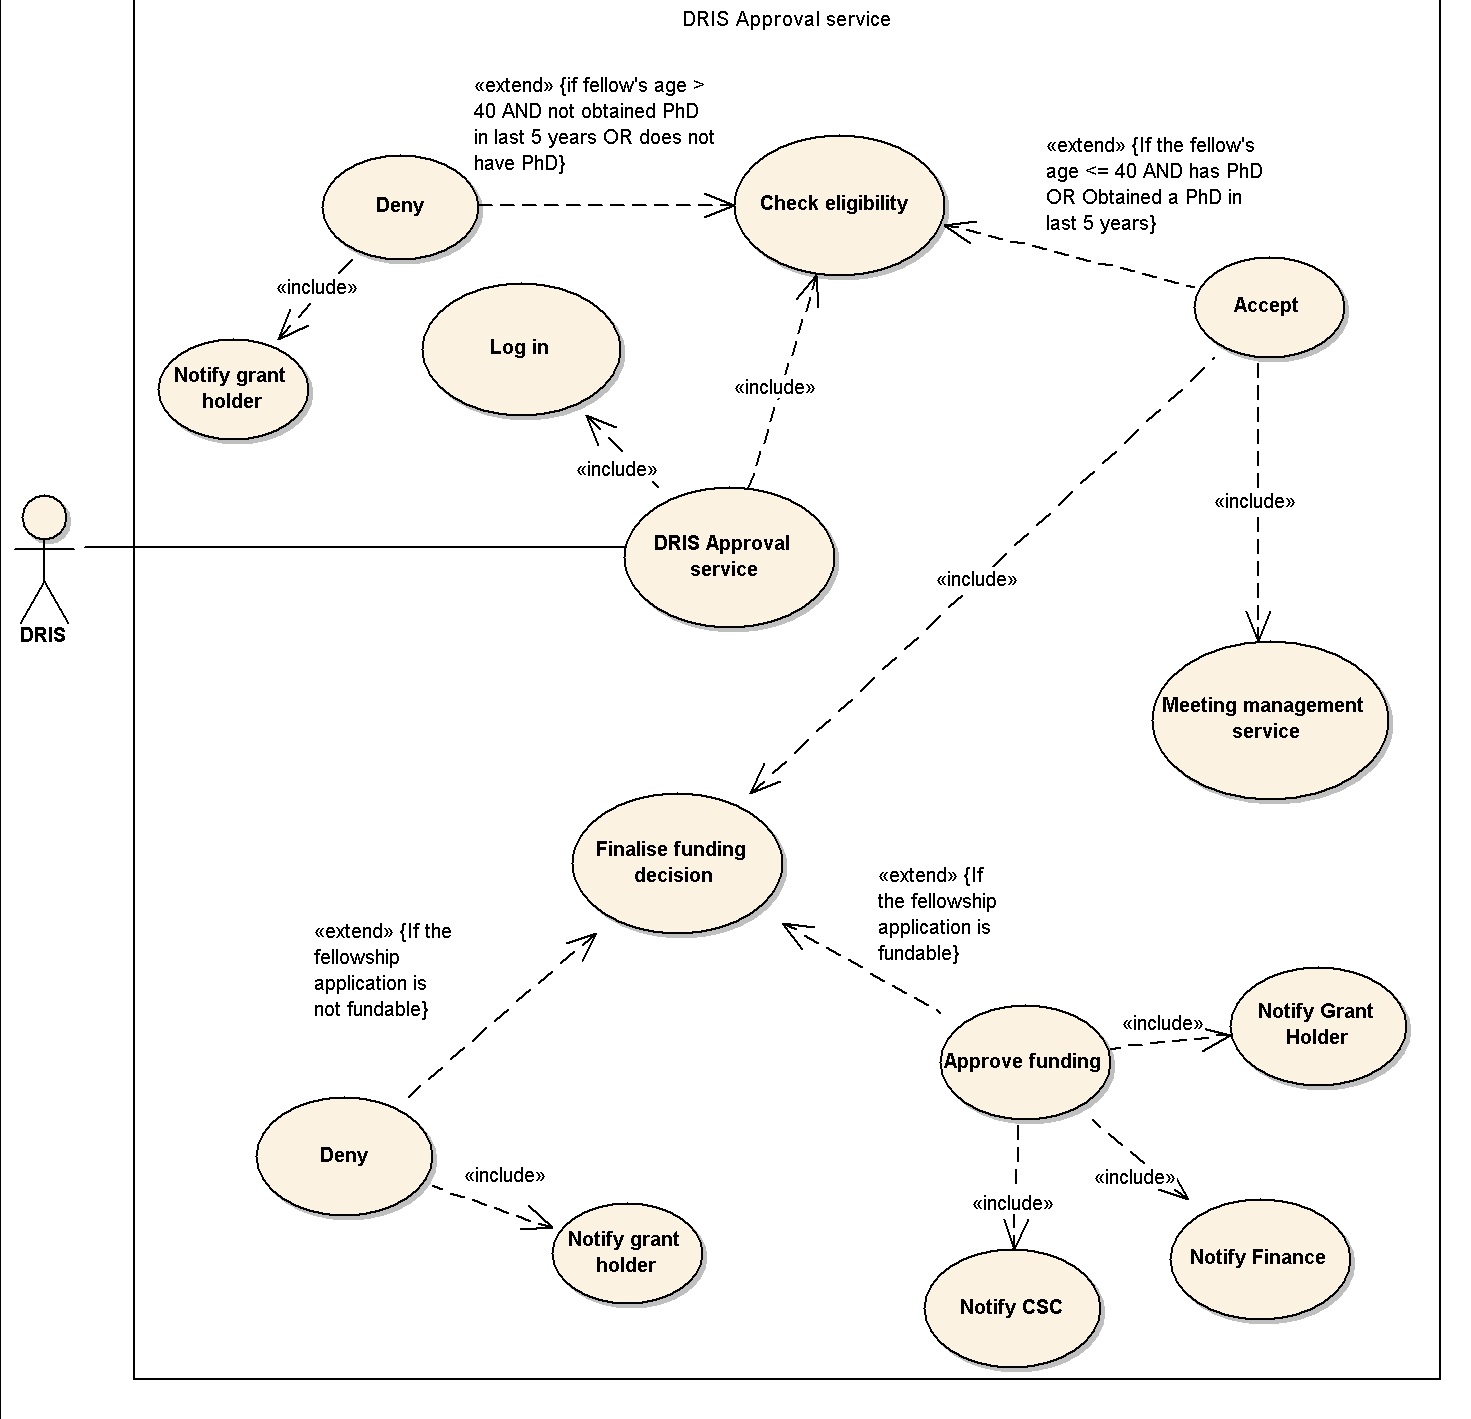
\includegraphics[scale=0.6]{./Pictures/Diagrams/Application/DRIS approval service.jpg}}
				\caption{Use case diagram of DRIS approval service}
			\end{figure}
			
			\begin{figure}[H]
				\centering				
				\framebox{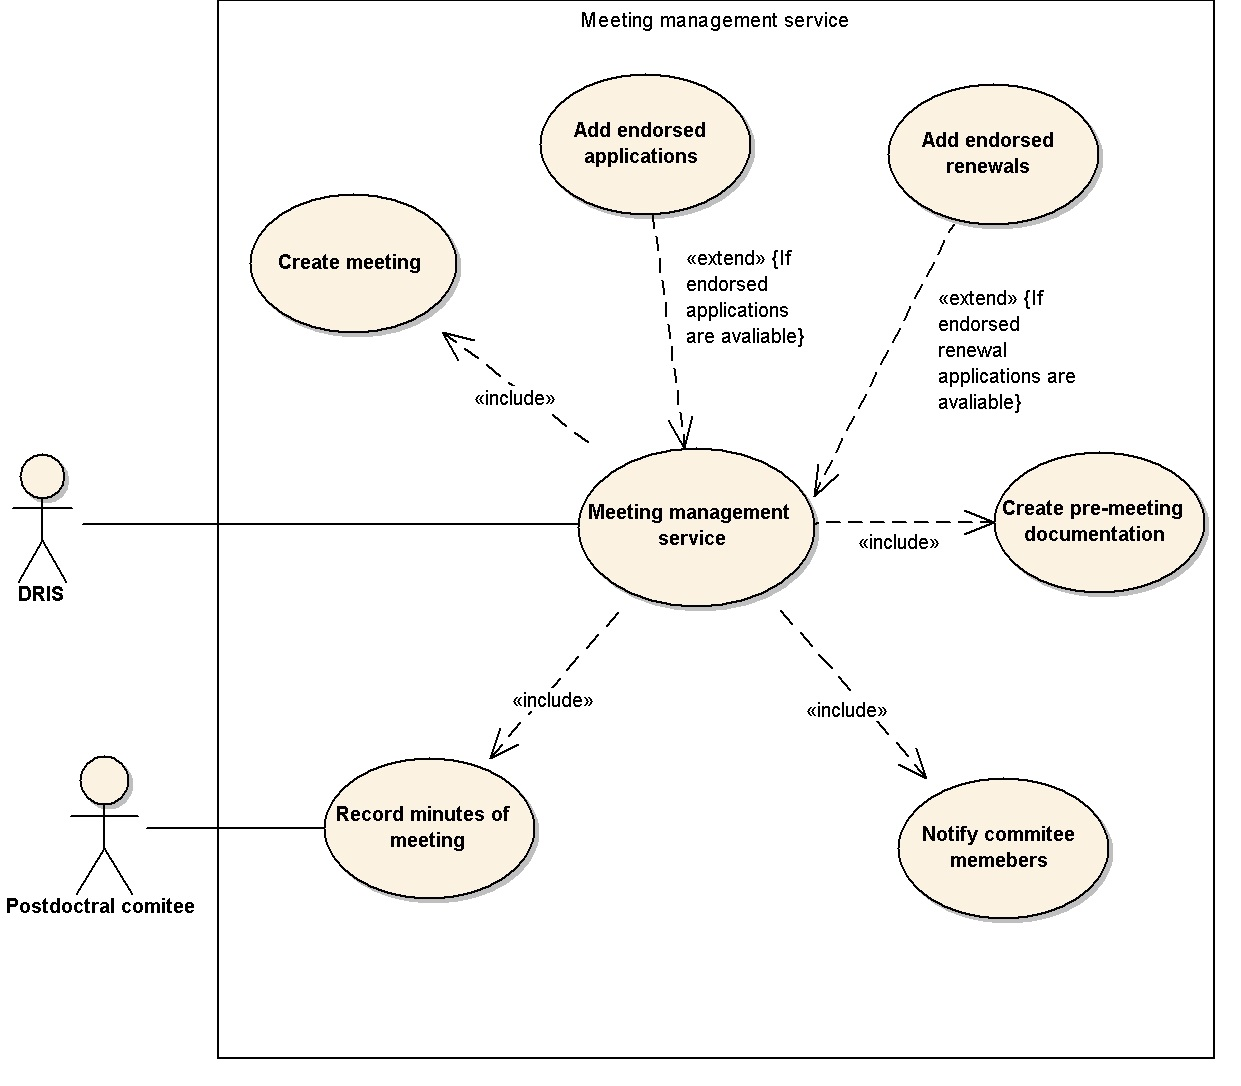
\includegraphics[scale=0.6]{./Pictures/Diagrams/Application/Meeting management service.jpg}}
				\caption{Use case diagram of Meeting management service}
			\end{figure}
		
		\vspace{0.2in}
		\subsubsection{Exclusions}
		\vspace{0.2in}
		Everything not included in this document in terms of scope is considered not in the scope of the project.
		\vspace{0.2in}
		
		\subsection{Required functionality} %Alfred
		\vspace{0.2in}
		The following sections will discuss the required functionality of all the major services handled by the system. Namely:
		\begin{itemize}
			\item Application service
			\item Report services
			\item Notification services
			\item User account management services			
		\end{itemize}
		
		%Use the use case diagrams to complete the requirements of each of the services in the format I provided
		\subsubsection{Application services}
		Th main user of these services will be the prospective fellows who wishes to track their application progress or renew or apply for a Post-Doctoral fellowship. Other stakeholders will only make use of certain sub-services which are provided under the Application services:
		
		\begin{itemize}
			\item New fellowship application service API:		
			\begin{enumerate}
				\item Account creation for new prospective fellows, referees and grant holders.
				\item All internal stakeholders should be able to log in with their PeopleSoft account details.				
				\item A prospective fellow should be able to open a new application. 
				\item A prospective fellow should be able to add their CV in the required format. 
				\item A prospective fellow should be able to specify their indented grant holder.
				%Please complete this in the same format				
			\end{enumerate}
			
			\item Fellowship renewal service API:
			\item Application progress viewer service API:
		\end{itemize}
		
		Once the steps are completed the applicants application is now under consideration. The applicant will also be able to see the status of the the applications current state through the whole application process.
		\subsubsection{Report services}
		The report use cases provides the uses for report generation such as the generation of an applications current status, the			
		\subsubsection{User account management services}
		The application will now go through a chain of various stakeholders, namely... , who will either approve or decline the application. If the application is declined, reason to why it was declined can be provided to allow the applicant to rectify the issue and continue with the application. If an application is approved, it will then be forward on to the next stakeholder in the system.
		\subsubsection{Notification services}
		Every participant is due to receive notifications regarding their actions every now and then.
		
		\vspace{0.2in}
		\subsection{Use case prioritization} %Alfred
		\vspace{0.2in}
		
		%Just prioritize each use case
		
		\vspace{0.2in}
		
		\subsection{Use case/Services contracts} %Mathys
		\vspace{0.2in}
		
		\begin{itemize}
		
		\item Preconditions:
			\begin{itemize}
				\item New fellowship application service [Fig 2.]: Can only be accessed if new applications are open. 
				\item Fellow ship renewal service [Fig 2.]: Can only be accessed if renewals are open.
				\item Application progress viewer service [Fig 2.]: Can only be accessed if user logged in with correct security permissions.
				\item View application progress [Fig 6.]: Can only be used if there are any applications made by the user.
			\end{itemize}
		\item Postconditions:
		\end{itemize}
		
		\vspace{0.2in}
		
		\subsection{Process specifications} %Alfred
		\vspace{0.2in}
		
		\vspace{0.2in}
		
		\subsection{Domain Objects} %Alfred
		\subsubsection{Overview}
		\begin{description}
			\item[Stakeholder] the full participants who administer the application process. Namely: 
				\begin{itemize}
					\item DRIS
					\item Dean's office
					\item Grant holder
					\item HOD
					\item Post-doctoral committee
					\item Prospective fellow
					\item Referee
				\end{itemize}
			\item[Application] which will be created by prospective fellow. Viewed and supplemented by other stakeholders who will either approve or deny the application.
			\item[Post-doctoral committee meetings] held to discuss issues relating to the Post-Doctoral system such as ranking and evaluating applicants.
		\end{description}
		\vspace{0.5in}
		\subsubsection{Stakeholder}
		All stakeholders, except referees, will have accounts which they use to log on to the system with a unique username and a predefined or user specified password.\linebreak \linebreak
		Grant holder are possibly rated researchers by the NRF and the system should not require the CV's of A and B rated researchers to be added to the system. The reason for this is that the CV's of such researchers are very long.
		\subsubsection{Application}
		Applications will contain the required info of a prospective fellow, e.g. CV and academic record, and who their researcher leader (grant holder) is. The status of the application will be accessible in reports for all stakeholders. The status will either be under consideration, denied or accepted.
		\subsubsection{Post-doctoral committee meetings}
		The post-doctoral committee will be assessing the applications and will evaluate and give an application a ranking.
		
	\newpage	
	\section{Open Issues:} %Everyone
	\vspace{0.2in}
	
	\begin{itemize}
		\item Theft or loss of mobile devices
		\item User errors like typing errors
		\item How will an applicant be allocated a student number?
		\item Should the system treat a prospective fellow in a unique class or a should all stakeholders be of the same class and be allocated different roles, as someone could work as a stakeholder but still want to apply?
		\item Automating a check for the rating of researchers.
		\item The CVs of A and B rated researchers was not added to save paper. Should we still not add it to keep it more convineint for the researchers?
	\end{itemize}
	
	
	\vspace{0.5in}
	
	\newpage
	\section{Glossary:} %Mathys
	\vspace{0.2in}
	
	\begin{itemize}
		
		
		\item \textbf{CV} - Curriculum Vita
		\item \textbf{PDF} - Portable Document Format file
		\item \textbf{NRF} - National Research Foundation 
		\item \textbf{HTML} - Hyper Text Mark-up Language
		 
	\end{itemize}	
		
	
	\vspace{0.5in}
		

\end{document}
